% We adopt the presentation from~\cite{barr1990category}, where a category is viewed as an unlabeled directed graph~\autorefbrackets{def:cat} equipped with two additional functions and their associated properties. In this framework, a homomorphism~\autorefbrackets{def:cat:homo} is simply another term for an arrow. To enhance readability, we utilize the concepts of spans and cospans. After introducing the notion of a commutative diagram~\autorefbrackets{def:cat:diagram}, we proceed to define the pushout~\autorefbrackets{def:cat:po_pb}. The construction of pushouts in the category \textbf{Graph} is also explain.
% To establish the categorical foundations necessary for our work, we recall key concepts such as monomorphisms, spans, cospans, commutative diagrams, and pushouts, following the presentation in~\cite{barr1990category}. We then focus on pushouts with monomorphisms within the category of graphs.
% We follow the presentation in~\cite{barr1990category}. We then focus on pushouts with monomorphisms within the category of graphs.
 
% cat def
\begin{definition}[Category \cite{pierce1991basic, barr1990category}]
    \label{def:cat}
    A \textbf{category} is an unlabeled graph \( C \) together with a total function \( u : C_0 \to C_1 \) and a partial function \( \star: C_1 \times C_1 \to C_1 \) such that 
        (i) for all edges \( f:X \to Y \) and \( g:Y \to Z \), the edge \( f \star g :X \to Z \) is defined; 
        (ii) for every node \( X \), \( u(X) \) is an edge from \( X \) to \( X \);
        (iii) for every \( f:X \to Y \), we have \(u(X) \star f = f = f \star u(Y)\);
        (iv) for all edges \( f \), \( g \) and \(h\), we have \( (f \star g) \star h = f \star (g \star h) \) whenever either side is defined.
    Edges are called \textbf{morphisms}. The function $\star$ is called \textbf{composition}. For all \( X \in C_0 \), the edge \( u(X) \) is denoted \( \operatorname{id}_X \) and is called the \textbf{identity} of the object \( X \).
    % \( C \) is called the \textbf{underlying graph} of the category \( \mathcal{C} \).
\end{definition} 

% cat notation * 
\begin{notation}
    The composition of morphisms \( f : X \mathop{\to} Y \) and \( g : Y \mathop{\to} Z \) is written in diagrammatic order as \( f \mathop{\star} g \), rather than in functional order \( g \circ f \). 
    % The advantage is that, when reading from left to right, the morphisms appear in the same order as in the corresponding diagram, making the notation more intuitive for visual reasoning.
\end{notation}  

\begin{definition}[Monomorphism~\cite{pierce1991basic,barr1990category}]
    \label{def:cat:homo}
    A morphism \( f : X \to Y \) is \textbf{monic} (or a \textbf{monomorphism}) if for all morphisms \( g \) and \( h \), if \( g \star f = h \star f \), then \( g = h \). A monomorphism is denoted by \( f : X \rightarrowtail Y \).
\end{definition} 

\begin{example}
    Labeled graphs and their homomorphisms forms a category, referred to as \textbf{Graph}. Its objects are labeled graphs, its morphisms are graph homomorphisms, and the monomorphisms are injective homomorphisms.
\end{example}

%span
\begin{definition}[Span~\cite{lowe2010graph}]
    An ordered pair \( (\alpha : A \mathop{\to} B,~\beta : A \mathop{\to} C) \) of morphisms with a common domain is called a \textbf{span}, denoted by \( B \overset{\alpha}{\leftarrow} A \overset{\beta}{\rightarrow} C \).
\end{definition}
%cospan
\begin{definition}[Cospan]
    An ordered pair \( (\beta' : B \to D,~\alpha' : C \to D) \) of morphisms with a common codomain is called a \textbf{cospan}, denoted by \( B \overset{\beta'}{\rightarrow} D \overset{\alpha'}{\leftarrow} C \). 
\end{definition} 
%diagram 

\begin{definition}[Diagram \cite{barr1990category}]
    \label{def:cat:diagram}
    Let \( G \) be an unlabeled graph. A \textbf{diagram} (in \( \mathcal{C} \) of shape \( G \)) is a homomorphism of unlabeled graphs \( h : G \to C \) where \( C \) is the underlying unlabeled graph of the category \( \mathcal{C} \). A diagram is \textbf{commutative} if, for all nodes \( u \), \( v \), and any two paths from \( u \) to \( v \) in the unlabeled graph \( G \):

    \begin{center}
    \resizebox{12cm}{!}{
        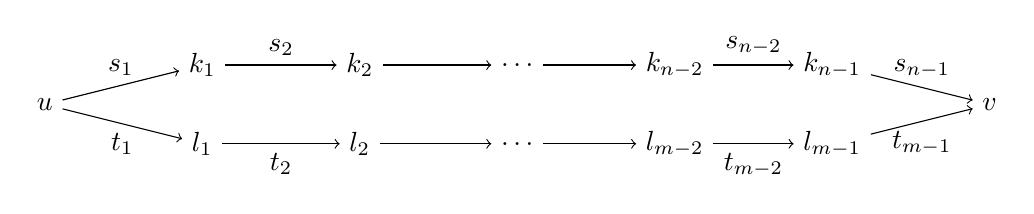
\begin{tikzpicture}
        \node (u) at (0,0) {\( u \)};
        \node (k1) at (2,0.5) {\( k_1 \)};
        \node (k2) at (4,0.5) {\( k_2 \)};
        \node (ketc) at (6,0.5) {\( \dots \)};
        \node (knm2) at (8,0.5) {\( k_{n-2} \)};
        \node (knm1) at (10,0.5) {\( k_{n-1} \)};
        \node (v) at (12,0) {\( v \)};
        \node (l1) at (2,-0.5) {\( l_1 \)};
        \node (l2) at (4,-0.5) {\( l_2 \)};
        \node (letc) at (6,-0.5) {\( \dots \)};
        \node (lnm2) at (8,-0.5) {\( l_{m-2} \)};
        \node (lnm1) at (10,-0.5) {\( l_{m-1} \)};
        \draw[->] (u) -- (k1) node [midway,above] {\( s_1 \)};
        \draw[->] (k1) -- (k2) node [midway,above] {\( s_2 \)};
        \draw[->] (k2) -- (ketc);
        \draw[->] (ketc) -- (knm2); 
        \draw[->] (knm2) -- (knm1) node[midway,above] {\( s_{n-2} \)}; 
        \draw[->] (knm1) -- (v) node[midway,above] {\( s_{n-1} \)}; 
        \draw[->] (u) -- (l1) node[midway,below] {\( t_1 \)};
        \draw[->] (l1) -- (l2) node[midway,below] {\( t_2 \)};
        \draw[->] (l2) -- (letc);
        \draw[->] (letc) -- (lnm2); 
        \draw[->] (lnm2) -- (lnm1) node[midway,below] {\( t_{m-2} \)}; 
        \draw[->] (lnm1) -- (v) node[midway,below] {\( t_{m-1} \)}; 
        \end{tikzpicture}
    }
    \end{center}
    \noindent
    the equality \( h(s_1) \star h(s_2) \star \dots  \star h(s_{n-1}) = h(t_1) \star h(t_2) \star \dots  \star h(t_{m-1}) \) holds.
\end{definition}

Pushouts play a central role in the double-pushout approach to graph rewriting considered in this thesis. The concepts and notation in this section follow the treatments of Pierce~\cite{pierce1991basic} and Barr and Wells~\cite{barr1990category}.
\begin{definition}
    \label{def:cat}
    A \textbf{category}\index{Category} is an unlabeled graph \( C \) together with a total function \( u : V(C)  \mathop{\to} E(C) \) and a partial function \( \star: E(C) \mathop{\times} E(C)  \mathop{\to} E(C) \) such that 
        \begin{itemize}
            \item for all edges \( f:X  \mathop{\to} Y \) and \( g:Y  \mathop{\to} Z \), the edge \( f \mathop{\star} g :X  \mathop{\to} Z \) is defined; 
            \item  for every node \( X \), \( u(X) \) is an edge from \( X \) to \( X \); 
            \item for every \( f:X  \mathop{\to} Y \), we have \(u(X) \mathop{\star} f \mathop{=} f \mathop{=} f \mathop{\star} u(Y)\);
            \item for all edges \( f \), \( g \) and \(h\), we have \( (f \mathop{\star} g) \mathop{\star} h \mathop{=} f \mathop{\star} (g \mathop{\star} h) \) whenever either side is defined.
        \end{itemize}
    Edges are called \textbf{morphisms}\index{Morphism}. The function $\star$ is called \textbf{composition}\index{Composition}. For all \( X \mathop{\in} V(C) \), the edge \( u(X) \) is denoted by \( \operatorname{id}_X \) and is called the \textbf{identity}~\index{Indentity} of the object \( X \).
    % \( C \) is called the \textbf{underlying graph} of the category \( \mathcal{C} \).
\end{definition}    
\begin{definition}
    A category \(\mathcal{C}\) is said to be \textbf{locally small}\index{Category!locally small} if for all objects \(X,Y\) in \(\mathcal{C}\), the collection $\opn{Hom}(X,Y)$\index{hom(@$\opn{Hom}(X,Y)$} of morphisms from \(X\) to \(Y\) is a set (called a \textbf{hom-set})~\index{Hom-set}. For a locally small category, $\opn{Mono}(X,Y)$\index{mono(@$\opn{Mono}(X,Y)$} denotes the set of all monomorphisms from $X$ to $Y$.
\end{definition}
\textbf{Throughout this section, fix a locally small category \( \mathcal{C} \).}
\begin{example}
    Consider the unlabeled graph shown below.
    %  in Figure~\ref{fig:preliminaries:category}. 
     It can be considered as a category where the objects are the nodes and the morphisms are the paths between nodes; composition is path concatenation. The identity of a node is the self-loop of the node. There are at least three morphisms from the left node to itself: the identity morphism (the self-loop), the path that traverses the self-loop twice, and the path that goes to the right node and back. 
        % \begin{figure}[H]
        % \centering
        \begin{center}
            \resizebox{0.4\textwidth}{!}{
        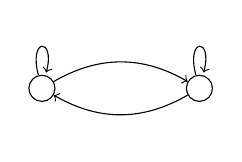
\begin{tikzpicture}
            \graphbox{}{0mm}{0mm}{32mm}{16mm}{-10mm}{-9mm}{
                \node[draw,circle] (1) at (0,0) {};
                \node[draw,circle] (2) at (2,0) {};
                \draw[->] (1) edge[loop above] node[midway, above] { } (1) ;
                \draw[->] (2) edge[loop above] node[midway, above] { } (2) ;
                \draw[->] (1) edge[bend left] node[midway, above] {}  (2)  ;
                \draw[->] (2) edge[bend left] node[midway, below] {} (1)   ;
            }
        \end{tikzpicture}
            }
    %     \caption{}
    %     \label{fig:preliminaries:category}
    % \end{figure}
        \end{center}
\end{example}

% cat notation * 
\begin{notation}
    The composition of morphisms \( f : X  \mathop{\to} Y \) and \( g : Y  \mathop{\to} Z \) is written in diagrammatic order as \( f \mathop{\star} g \), rather than in functional order \( g \circ f \) as is common in litterature. The advantage is that, when reading from left to right, the morphisms appear in the same order as in the corresponding diagram, making the reasoning accompanying diagrams more intuitive. 
\end{notation}  

\begin{definition} 
    \label{def:cat:homo}
    A morphism \( f : X  \mathop{\to} Y \) is said to be a \textbf{monomorphism}\index{Monomorphism} (is \textbf{monic}\index{Monic}) if given any morphisms \( g,h: Z  \mathop{\to} X  \), \( g \mathop{\star} f \mathop{=} h \mathop{\star} f \) implies \( g \mathop{=} h \). 
    In this case, we write $f : X \rightarrowtail Y$\index{a@$\rightarrowtail$} to indicate that $f$ is a monomorphism.
\end{definition} 

When visualizing a monomorphism, we often use $\rightarrowtail$ instead of $\to$ to emphasize that it is monic. For example, a monomorphism of labeled graphs can be represented as follows:
\begin{center}
        \resizebox{0.7\textwidth}{!}{
        \begin{tikzpicture}
            \graphbox{$K$}{40mm}{0mm}{24mm}{15mm}{2mm}{-5mm}{
                \coordinate (o) at (5mm,-3mm); 
                \node[draw,circle] (l1) at ($(o)+(-10mm,0mm)$) {1};
                \node[draw,circle] (l2) at ($(l1)+(1,0)$) {2};
            }    
            \graphbox{$R$}{70mm}{0mm}{45mm}{15mm}{2mm}{-5mm}{
                \coordinate (o) at (-5mm,-3mm); 
                \node[draw,circle] (l1) at ($(o)+(-10mm,0mm)$) {1};
                \node[draw,circle] (l2) at ($(l1)+(3,0)$) {2};
                \node[draw,circle] (l3) at ($(l1)+(1,0)$) {4};
                \node[draw,circle] (l4) at ($(l1)+(2,0)$) {5};
                \draw[->] (l1) -- (l3) node[midway,above] {$a$};
                \draw[->] (l3) -- (l4) node[midway,above] {$b$};
                \draw[->] (l4) -- (l2) node[midway,above] {$a$};
            }    
            \node () at (67mm,-8mm) {$\rightarrowtail$};
        \end{tikzpicture}
        }
    \end{center}

\begin{example}
    \index{set@\(\mathbf{Set}\)}\index{Category!set}
The category \(\mathbf{Set}\) has sets as objects and total functions between them as morphisms. For \(f\mathop{\colon} A \mathop{\to} B\) and \(g\mathop{\colon} B \mathop{\to} C\), composition is given by \(g\circ f\), and the identity morphism on a set \(A\) is the identity function \(\mathrm{id}_A\).
\end{example}

\begin{example} 
    Finite labeled graphs and their homomorphisms form a category, hereafter denoted by \textbf{Graph}\index{graph@\textbf{Graph}}\index{Category!graph}. Its objects are labeled graphs, its morphisms are graph homomorphisms, and the monomorphisms are homomorphisms. 
    $\textbf{Graph}$ is locally small. 
\end{example}

% \begin{definition}[Span \cite{lowe2010graph}]
%     A pair \( (\alpha : A  \mathop{\to} B,~\beta : A  \mathop{\to} C) \) of morphisms with a common domain is called a \textbf{span}, denoted by \( B \overset{\alpha}{\leftarrow} A \overset{\beta}{\rightarrow} C \).
% \end{definition}
 
% \begin{definition}[Cospan]
%     A pair \( (\beta' : B  \mathop{\to} D,~\alpha' : C  \mathop{\to} D) \) of morphisms with a common codomain is called a \textbf{cospan}, denoted by \( B \overset{\beta'}{\rightarrow} D \overset{\alpha'}{\leftarrow} C \). 
% \end{definition} 
A span (resp. cospan) is a couple of morphisms with a common domain (resp. codomain).
\begin{definition}
An ordered pair \((\alpha : A  \mathop{\to} B,\, \beta : A  \mathop{\to} C)\) of morphisms with a common domain is called a \textbf{span}\index{Span} \cite{lowe2010graph}, denoted by
\(
B \overset{\alpha}{\leftarrow} A \overset{\beta}{\rightarrow} C
\). 
% An example of a span $(\alpha, \beta)$ is shown below.
Likewise, an ordered pair \((\beta' : B  \mathop{\to} D,\, \alpha' : C  \mathop{\to} D)\) of morphisms with a common codomain is called a \textbf{cospan}\index{Cospan}, denoted by
\(
B \overset{\beta'}{\rightarrow} D \overset{\alpha'}{\leftarrow} C
\). 
\end{definition}
\begin{example}
Consider the diagram below in the category \textbf{Graph}, where the numbers inside nodes and the subgraphs in different colors illustrate how the morphisms map nodes and edges. $(\alpha, \beta)$ is a span, and $(\beta', \alpha')$ is a cospan.


\begin{center}
        \resizebox{0.8\textwidth}{!}{
        \begin{tikzpicture} 
            \graphbox{\( L \)}{40mm}{20mm}{34mm}{12mm}{2mm}{2mm}{
                \coordinate (o) at (0mm,-8mm); 
                \node[draw,circle] (l1) at ($(o)+(-10mm,0mm)$) {1};
                \node[draw,circle] (l2) at ($(l1)+(2,0)$) {2};
                \node[draw,circle,red] (l3) at ($(l1)+(1,0)$) {3};
                \draw[->,red] (l1) -- (l3) node[midway,above] {$a$};
                \draw[->,red] (l3) -- (l2) node[midway,above] {$a$};
            } 
    
            \graphbox{\( K \)}{0mm}{0mm}{34mm}{12mm}{2mm}{2mm}{
                \coordinate (o) at (0mm,-8mm); 
                \node[draw,circle] (l1) at ($(o)+(-10mm,0mm)$) {1};
                \node[draw,circle] (l2) at ($(l1)+(2,0)$) {2};
            }  
            \graphbox{\(G\)}{90mm}{5mm}{34mm}{24mm}{2mm}{-3mm}{
                \coordinate (o) at (0mm,-5mm); 
                \node[draw,circle] (l1) at ($(o)+(-10mm,0mm)$) {1};
                \node[draw,circle] (l2) at ($(l1)+(2,0)$) {2};
                \node[draw,circle,red] (l3) at ($(l1)+(1,0)$) {3};
                \node[draw,circle,blue] (l4) at ($(l2)+(0,-1)$) {6};
                \draw[->,red] (l1) -- (l3) node[midway,above] {$a$};
                \draw[->,red] (l3) -- (l2) node[midway,above] {$a$};
                \draw[->,blue] (l2) -- (l4) node[midway,right] {$a$};
                \node[draw,circle,blue] (l6) at ($(l1)+(0,-1)$) {7};
                \draw[<-,blue] (l1) -- (l6) node[midway,left] {$a$};
                \draw[->,blue] (l2) edge[out=-135,in=-45]node[midway,below] {$a$} (l1) ;
            }   
     
            \graphbox{\( C \)}{40mm}{-20mm}{34mm}{24mm}{2mm}{-3mm}{
                \coordinate (o) at (0mm,-5mm); 
                \node[draw,circle] (l1) at ($(o)+(-10mm,0mm)$) {1};
                \node[draw,circle] (l2) at ($(l1)+(2,0)$) {2};
                \node[draw,circle,blue] (l4) at ($(l2)+(0,-1)$) {6};
                \draw[->,blue] (l2) -- (l4) node[midway,right] {$a$};
                \draw[->,blue] (l2) edge[out=-135,in=-45]node[midway,below] {$a$} (l1) ;
                \node[ draw,circle,blue] (l6) at ($(l1)+(0,-1)$) {7};
                \draw[<-,blue] (l1) -- (l6) node[midway,left] {$a$};
            }      
            % K to L
            \draw[->] (17mm,5mm) -- node[above] {$\alpha$} (37mm,15mm);
            % C to G
            \draw[->] (76mm,-28mm)-- node[below] {$\alpha'$} (104mm,-21mm) ;
            % K to C
            \draw[->] (17mm,-17mm) -- node[below] {$\beta$} (37mm,-28mm);
            % L to G
            \draw[->] (76mm,16mm) -- node[above] {$\beta'$} (104mm,7mm);
            % \node () at (57mm,-6mm) {$PO$};
        \end{tikzpicture}
        }
    \end{center}
\end{example}

\begin{definition}[\cite{barr1990category}]
    \label{def:cat:diagram}
    Let $\mathcal{C}$ be a category, and \( G \) an unlabeled graph. A \textbf{diagram}\index{Diagram} (of shape \( G \)) is a homomorphism of unlabeled graphs \( h : G  \mathop{\to} \mathcal{C} \) where \( \mathcal{C} \) is considered as an unlabeled graph. A diagram is said to be \textbf{commutative}\index{Diagram!commutative} if, for all nodes \( u \), \( v \), and any two paths from \( u \) to \( v \) in the unlabeled graph \( G \):

    \begin{center}
    \resizebox{12cm}{!}{
        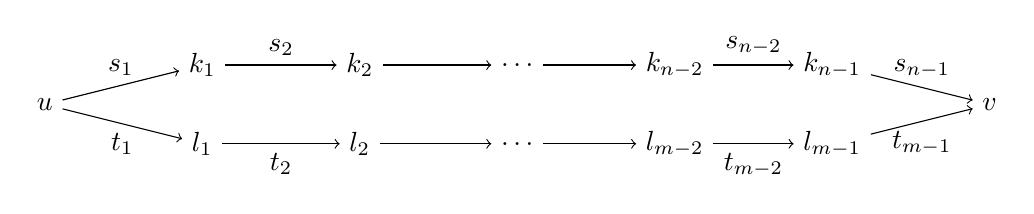
\begin{tikzpicture}
        \node (u) at (0,0) {\( u \)};
        \node (k1) at (2,0.5) {\( k_1 \)};
        \node (k2) at (4,0.5) {\( k_2 \)};
        \node (ketc) at (6,0.5) {\( \dots \)};
        \node (knm2) at (8,0.5) {\( k_{n-2} \)};
        \node (knm1) at (10,0.5) {\( k_{n-1} \)};
        \node (v) at (12,0) {\( v \)};
        \node (l1) at (2,-0.5) {\( l_1 \)};
        \node (l2) at (4,-0.5) {\( l_2 \)};
        \node (letc) at (6,-0.5) {\( \dots \)};
        \node (lnm2) at (8,-0.5) {\( l_{m-2} \)};
        \node (lnm1) at (10,-0.5) {\( l_{m-1} \)};
        \draw[->] (u) -- (k1) node [midway,above] {\( s_1 \)};
        \draw[->] (k1) -- (k2) node [midway,above] {\( s_2 \)};
        \draw[->] (k2) -- (ketc);
        \draw[->] (ketc) -- (knm2); 
        \draw[->] (knm2) -- (knm1) node[midway,above] {\( s_{n-2} \)}; 
        \draw[->] (knm1) -- (v) node[midway,above] {\( s_{n-1} \)}; 
        \draw[->] (u) -- (l1) node[midway,below] {\( t_1 \)};
        \draw[->] (l1) -- (l2) node[midway,below] {\( t_2 \)};
        \draw[->] (l2) -- (letc);
        \draw[->] (letc) -- (lnm2); 
        \draw[->] (lnm2) -- (lnm1) node[midway,below] {\( t_{m-2} \)}; 
        \draw[->] (lnm1) -- (v) node[midway,below] {\( t_{m-1} \)}; 
        \end{tikzpicture}
    }
    \end{center}
    \noindent
    the equality \( h(s_1) \mathop{\star} h(s_2) \mathop{\star} \dots  \mathop{\star} h(s_{n-1}) \mathop{=} h(t_1) \mathop{\star} h(t_2) \mathop{\star} \dots  \mathop{\star} h(t_{m-1}) \) holds.
\end{definition}

\begin{example}
    A commutative diagram in the category \textbf{Graph} of finite, directed, edge-labeled multigraphs is illustrated below. The numbers inside nodes and the subgraphs in different colors illustrate how the morphisms map nodes and edges. 
     The symbol $\mathop{=}$ in the center of the diagram
    is used to indicate that the diagram is commutative,
    i.e. the composition of morphisms along every path from node 1 to node 2 is the same.
    \begin{center}
        \resizebox{0.8\textwidth}{!}{
        \begin{tikzpicture} 
            \graphbox{\( L \)}{40mm}{20mm}{34mm}{12mm}{2mm}{2mm}{
                \coordinate (o) at (0mm,-8mm); 
                \node[draw,circle] (l1) at ($(o)+(-10mm,0mm)$) {1};
                \node[draw,circle] (l2) at ($(l1)+(2,0)$) {2};
                \node[draw,circle,red] (l3) at ($(l1)+(1,0)$) {3};
                \draw[->,red] (l1) -- (l3) node[midway,above] {$a$};
                \draw[->,red] (l3) -- (l2) node[midway,above] {$a$};
            } 
    
            \graphbox{\( K \)}{0mm}{0mm}{34mm}{12mm}{2mm}{2mm}{
                \coordinate (o) at (0mm,-8mm); 
                \node[draw,circle] (l1) at ($(o)+(-10mm,0mm)$) {1};
                \node[draw,circle] (l2) at ($(l1)+(2,0)$) {2};
            }  
            \graphbox{\(G\)}{90mm}{5mm}{34mm}{24mm}{2mm}{-3mm}{
                \coordinate (o) at (0mm,-5mm); 
                \node[draw,circle] (l1) at ($(o)+(-10mm,0mm)$) {1};
                \node[draw,circle] (l2) at ($(l1)+(2,0)$) {2};
                \node[draw,circle,red] (l3) at ($(l1)+(1,0)$) {3};
                \node[draw,circle,blue] (l4) at ($(l2)+(0,-1)$) {6};
                \draw[->,red] (l1) -- (l3) node[midway,above] {$a$};
                \draw[->,red] (l3) -- (l2) node[midway,above] {$a$};
                \draw[->,blue] (l2) -- (l4) node[midway,right] {$a$};
                \node[draw,circle,blue] (l6) at ($(l1)+(0,-1)$) {7};
                \draw[<-,blue] (l1) -- (l6) node[midway,left] {$a$};
                \draw[->,blue] (l2) edge[out=-135,in=-45]node[midway,below] {$a$} (l1) ;
            }   
     
            \graphbox{\( C \)}{40mm}{-20mm}{34mm}{24mm}{2mm}{-3mm}{
                \coordinate (o) at (0mm,-5mm); 
                \node[draw,circle] (l1) at ($(o)+(-10mm,0mm)$) {1};
                \node[draw,circle] (l2) at ($(l1)+(2,0)$) {2};
                \node[draw,circle,blue] (l4) at ($(l2)+(0,-1)$) {6};
                \draw[->,blue] (l2) -- (l4) node[midway,right] {$a$};
                \draw[->,blue] (l2) edge[out=-135,in=-45]node[midway,below] {$a$} (l1) ;
                \node[ draw,circle,blue] (l6) at ($(l1)+(0,-1)$) {7};
                \draw[<-,blue] (l1) -- (l6) node[midway,left] {$a$};
            }      
            % K to L
            \draw[->] (17mm,5mm) -- node[above] {$\alpha$} (37mm,15mm);
            % C to G
            \draw[->] (76mm,-28mm)-- node[below] {$\alpha'$} (104mm,-21mm) ;
            % K to C
            \draw[->] (17mm,-17mm) -- node[below] {$\beta$} (37mm,-28mm);
            % L to G
            \draw[->] (76mm,16mm) -- node[above] {$\beta'$} (104mm,7mm);
            \node () at (57mm,-6mm) {$\mathop{=}$};
        \end{tikzpicture}
        }
    \end{center}
\end{example}

\begin{notation}   
    When the context makes it clear, \( h_{AB} \) denotes a morphism \( h : A  \mathop{\to} B \), and we refer to diagrams by listing their nodes, as is standard in geometry. 
    % For example, the diagram shown in Definition~\ref{def:cat:po} is denoted by \( ACDB \) or \( ABDC \).
\end{notation}   

The pushout is a construction in category theory that can often be thought of as the construction of a new structure from two given structures by gluing them along a common interface structure.
\begin{definition}
    \label{def:cat:po} 
    A \textbf{pushout}\index{Pushout} of a span \( B \overset{\alpha}{\leftarrow} A \overset{\beta}{\rightarrow} C \), shown in the following diagram,
    %  in Figure~\ref{fig:preliminaries:pushout_sdfkjasdlgjfl}
    is defined as a cospan \( B \overset{\beta'}{\rightarrow} D \overset{\alpha'}{\leftarrow} C \) such that the following conditions hold:
    \begin{itemize}
        \item \( \alpha \mathop{\star} \beta' \mathop{=} \beta \mathop{\star} \alpha' \),
        \item for every cospan \( B \overset{\gamma'}{\rightarrow} E \overset{\gamma}{\leftarrow} C \), if \( \alpha \mathop{\star} \gamma' \mathop{=} \beta \mathop{\star} \gamma \) holds, then there is a unique morphism \(\delta : D  \mathop{\to} E\) such that \( \gamma' \mathop{=} \beta' \mathop{\star} \delta \) and \( \gamma \mathop{=} \alpha' \mathop{\star} \delta \).
    \end{itemize} 
    \begin{center}
        \resizebox{0.45\textwidth}{!}{
            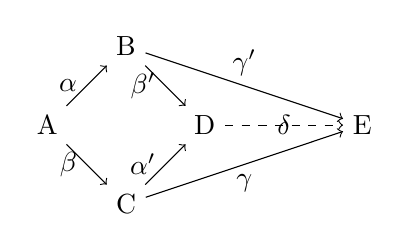
\begin{tikzpicture}
                    \node (i) at (0,0) {A};
                    \node (r) at (1,1) {B};
                    \node (c) at (1,-1) {C};
                    \node (h) at (2,0) {D};
                    % \node () at (1,-1) {\( \Delta \)};
                    \draw[->]  (i) -- (r) node [midway,left] {$ \alpha $};
                    \draw[->] (c) -- (h) node [midway,left] {$ \alpha' $};
                    \draw[->] (r) -- (h) node[midway, left] {$ \beta' $};
                    \draw[->] (i) -- (c) node[midway, left] {$ \beta $};
                    \node (d') at (4,0) {E};
                    \draw[->] (c) -- (d') node [midway,below]{$ \gamma $};
                    \draw[->] (r) -- (d') node [midway,above]{$ \gamma' $};
                    \draw[->,dashed] (h) -- (d') node [midway]{$ \delta $};
                \end{tikzpicture}
        }
            \end{center}
The diagram involving \( (\alpha, \beta, \alpha', \beta') \) is called a \textbf{pushout square}\index{Pushout!square}, or simply a \textbf{pushout}, with \(D\) as the \textbf{pushout object}\index{Pushout!object}. The existence of a unique morphism is known as the \textbf{universal mapping property of the pushout}\index{Pushout!universal mapping property}.
\end{definition} 

\begin{example}
    \label{ex:cat:posfjsdlkgja}
     Pushouts of a span always exist in \(\mathbf{Set}\), and (up to isomorphism) can be described as follows. Let
    \( B \overset{\alpha}{\leftarrow} A \overset{\beta}{\rightarrow} C \) be a span. Its pushout is the cospan \( B \overset{\beta'}{\rightarrow} D \overset{\alpha'}{\leftarrow} C \) where the pushout object of \((\alpha,\beta)\) is the quotient set
    \[
    D \;=\; (B\mathop{+}C)/{\sim}
    \]
    where \(B\mathop{+}C\) denotes the disjoint union of $B$ and $C$ and \(\sim\) is the smallest equivalence relation that includes \(\set{(\alpha(a),\beta(b))\mid a \mathop{\in} A }\). The maps
    \(\beta' \mathop{\colon} B \mathop{\to} D\) and \(\alpha' \mathop{\colon} C \mathop{\to} D\) send each element to its equivalence class.

    For example, consider the functions \(\alpha\) and \(\beta\) in the category \(\mathbf{Set}\) in the diagram, illustrated in Figure~\ref{fig:preliminaries:a_rewriting_step_dfjalsdkjflg}.
    In this diagram, each set is drawn as a box and its elements are represented by circles. The numbers inside circles indicate how the functions map those elements.
    \begin{figure}[H]
      \centering 
      \resizebox{0.6\textwidth}{!}{
      \begin{tikzpicture}
          \graphbox{\( A\)}{40mm}{-3mm}{34mm}{12mm}{2mm}{2mm}{
              \coordinate (o) at (0mm,-8mm); 
              \node[draw,circle] (l1) at ($(o)+(-10mm,0mm)$) {1};
              \node[draw,circle] (l2) at ($(l1)+(2,0)$) {2};
          }  
          \graphbox{\( B \)}{80mm}{-3mm}{45mm}{12mm}{2mm}{2mm}{
              \coordinate (o) at (-5mm,-8mm); 
              \node[draw,circle] (l1) at ($(o)+(-10mm,0mm)$) {1};
              \node[draw,circle] (l2) at ($(l1)+(3,0)$) {2};
              \node[draw,circle] (l3) at ($(l1)+(1,0)$) {4};
          }     
          \graphbox{\( C  \)}{40mm}{-22mm}{34mm}{22mm}{2mm}{-3mm}{
              \coordinate (o) at (0mm,-3mm); 
              \node[draw,circle] (l1) at ($(o)+(-10mm,0mm)$) {1};
              \node[draw,circle] (l2) at ($(l1)+(2,0)$) {2};
              \node[ draw,circle] (l6) at ($(l1)+(0,-1)$) {3};
          }    
          \graphbox{\( D \)}{80mm}{-22mm}{45mm}{22mm}{2mm}{-3mm}{
              \coordinate (o) at (-5mm,-3mm); 
              \node[draw,circle] (l1) at ($(o)+(-10mm,0mm)$) {1};
              \node[draw,circle] (l2) at ($(l1)+(3,0)$) {2};
              \node[draw,circle] (l3) at ($(l1)+(1,0)$) {4};
              \node[ draw,circle] (l6) at ($(l1)+(0,-1)$) {3};
          }    
          \node () at (77mm,-8mm) {\( \overset{\alpha}{\rightarrow} \)}; % K -> R
          \node () at (58mm,-18mm) {\( \beta\downarrow \)};
          \node () at (102mm,-18mm) {\( \beta'\downarrow \)};
          \node () at (77mm,-33mm) {\( \overset{\alpha'}{\rightarrow} \)}; % C -> H
      \end{tikzpicture}
      }
      \caption{}
      \label{fig:preliminaries:a_rewriting_step_dfjalsdkjflg}
  \end{figure}
    Throughout this example, an element labeled \(n\) in a set \(X\) is denoted by \(n_X\) to avoid ambiguity.        
    The binary relation \(\sim\) is the reflexive, symmetric and transitive closure of the binary relation $\{(1_B,1_C),(2_B,2_C)\}$.
 
    The disjoint union of \(B\) and \(C\) is
    \[ 
    D' \mathop{=} \{1_B,2_B,4_B,1_C,2_C,3_C\},
    \]
    and the quotient set is
    \[
    D'/\sim \mathop{=} \{[1_B],[2_B],[3_C],[4_B]\},
    \]
    where $[x]$ denotes the equivalence class of the element \(x\).
    We have \([1_C]=[1_B]\) and \([2_C]=[2_B]\), and the maps
    \(\beta'' \mathop{\colon} B \mathop{\to} D'\) and \(\alpha'' \mathop{\colon} C \mathop{\to} D'\) send each element to its equivalence class. Note that \(\{[1_B],[2_B],[3_C],[4_B]\}\) is isomorphic to \(D\), shown in Figure~\ref{fig:preliminaries:a_rewriting_step_dfjalsdkjflg}, which is expected because the pushout of a span is unique up to isomorphism.
\end{example}

\begin{proposition}{\cite[p.188]{corradini1997algebraic}}
    \label{prop:pushout_graph_always_exists}
    In category \textbf{Graph}, the pushout of two arrows always exists: It can be computed componentwise (as a pushout in \textbf{Set}) for the nodes and for the edges, and the source, target, and labeling mappings are uniquely determined.
\end{proposition}

\begin{example}
    The diagram in the category \textbf{Graph} shown below
    %  in Figure~\ref{fig:preliminaries:pushout_injective} 
     is a pushout square. The numbers inside nodes and the subgraphs in different colors illustrate how the morphisms map nodes and edges. In this example, both $\alpha$ and $\beta$ are injective morphisms. Therefore, the pushout object $G$ can be constructed easily by taking the interface graph $K$ and adding elements from $L$ and $C$ which are not present in $K$.
    % \begin{figure}[H]
    %     \centering
    \begin{center}
        \resizebox{0.8\textwidth}{!}{
        \begin{tikzpicture} 
            \graphbox{\( L \)}{40mm}{15mm}{34mm}{12mm}{2mm}{2mm}{
                \coordinate (o) at (0mm,-8mm); 
                \node[draw,circle] (l1) at ($(o)+(-10mm,0mm)$) {1};
                \node[draw,circle] (l2) at ($(l1)+(2,0)$) {2};
                \node[draw,circle,red] (l3) at ($(l1)+(1,0)$) {3};
                \draw[->,red] (l1) -- (l3) node[midway,above] {$a$};
                \draw[->,red] (l3) -- (l2) node[midway,above] {$a$};
            } 
    
            \graphbox{\( K \)}{0mm}{0mm}{34mm}{12mm}{2mm}{2mm}{
                \coordinate (o) at (0mm,-8mm); 
                \node[draw,circle] (l1) at ($(o)+(-10mm,0mm)$) {1};
                \node[draw,circle] (l2) at ($(l1)+(2,0)$) {2};
            }  
            \graphbox{\(G  \)}{90mm}{5mm}{34mm}{24mm}{2mm}{-3mm}{
                \coordinate (o) at (0mm,-5mm); 
                \node[draw,circle] (l1) at ($(o)+(-10mm,0mm)$) {1};
                \node[draw,circle] (l2) at ($(l1)+(2,0)$) {2};
                \node[draw,circle,red] (l3) at ($(l1)+(1,0)$) {3};
                \node[draw,circle,blue] (l4) at ($(l2)+(0,-1)$) {6};
                \draw[->,red] (l1) -- (l3) node[midway,above] {$a$};
                \draw[->,red] (l3) -- (l2) node[midway,above] {$a$};
                \draw[->,blue] (l2) -- (l4) node[midway,right] {$a$};
                \node[draw,circle,blue] (l6) at ($(l1)+(0,-1)$) {7};
                \draw[<-,blue] (l1) -- (l6) node[midway,left] {$a$};
                \draw[->,blue] (l2) edge[out=-135,in=-45]node[midway,below] {$a$} (l1) ;
            }   
     
            \graphbox{\( C \)}{40mm}{-15mm}{34mm}{24mm}{2mm}{-3mm}{
                \coordinate (o) at (0mm,-5mm); 
                \node[draw,circle] (l1) at ($(o)+(-10mm,0mm)$) {1};
                \node[draw,circle] (l2) at ($(l1)+(2,0)$) {2};
                \node[draw,circle,blue] (l4) at ($(l2)+(0,-1)$) {6};
                \draw[->,blue] (l2) -- (l4) node[midway,right] {$a$};
                \draw[->,blue] (l2) edge[out=-135,in=-45]node[midway,below] {$a$} (l1) ;
                \node[ draw,circle,blue] (l6) at ($(l1)+(0,-1)$) {7};
                \draw[<-,blue] (l1) -- (l6) node[midway,left] {$a$};
            }      
            % K to L
            \draw[>->] (17mm,5mm) -- node[above] {$\alpha$} (37mm,10mm);
            % C to G
            \draw[>->] (76mm,-28mm)-- node[below] {$\alpha'$} (104mm,-21mm) ;
            % K to C
            \draw[>->] (17mm,-17mm) -- node[below] {$\beta$} (37mm,-28mm);
            % L to G
            \draw[>->] (76mm,10mm) -- node[above] {$\beta'$} (104mm,7mm);
            \node () at (57mm,-6mm) {$PO$};
        \end{tikzpicture}
        }
    \end{center}
    %     \caption{Pushout square with injective morphisms.}
    %     \label{fig:preliminaries:pushout_injective}
    % \end{figure}
\end{example}

\begin{example}
    \label{ex:cat:pushout_non_injective_ssss}
    Consider the diagram in the category \textbf{Graph} shown below, where the numbers inside nodes and the subgraphs in different colors illustrate how the morphisms map nodes and edges. 
    % The diagram 
    % in Figure~\ref{fig:preliminaries:pushout_non_injective} is a pushout square in the category \textbf{Graph}. 
    In this example, $\beta$ is not injective. Therefore, some elements are merged in the pushout object $G$.

    % \begin{figure}[H]
    %     \centering 
    \begin{center}
        \resizebox{0.8\textwidth}{!}{
        \begin{tikzpicture} 
            \graphbox{\( L \)}{40mm}{20mm}{34mm}{20mm}{2mm}{2mm}{
                \coordinate (o) at (0mm,-11mm); 
                \node[draw,circle] (l1) at ($(o)+(-10mm,0mm)$) {1};
                \node[draw,circle] (l2) at ($(l1)+(2,0)$) {2};
                \draw[->,red] (l2) edge[out=-135,in=-45]node[midway,below] {$a$} (l1) ;
                \node[draw,circle,red] (l3) at ($(l1)+(1,0)$) {3};
                \draw[->,red] (l1) -- (l3) node[midway,above] {$a$};
                \draw[->,red] (l3) -- (l2) node[midway,above] {$a$};
            } 
    
            \graphbox{\( K \)}{0mm}{0mm}{34mm}{12mm}{2mm}{2mm}{
                \coordinate (o) at (0mm,-8mm); 
                \node[draw,circle] (l1) at ($(o)+(-10mm,0mm)$) {1};
                \node[draw,circle] (l2) at ($(l1)+(2,0)$) {2};
            }  
            \graphbox{\(G  \)}{90mm}{10mm}{34mm}{40mm}{2mm}{-3mm}{
                \coordinate (o) at (0mm,-20mm); 
                 \node[draw,circle] (l1) at ($(o)+(0,0)$) {1\ 2};
                % \node[draw,circle] (l1) at ($(o)+(-10mm,0mm)$) {1};
                % \node[draw,circle] (l2) at ($(l1)+(2,0)$) {2};
                \draw[->,red] (l1) edge[loop below] node[midway, below] {$a$} (l1) ;
                \node[draw,circle,red] (l3) at ($(l1)+(0,1.4)$) {3};
                \node[draw,circle,blue] (l4) at ($(l1)+(1,-1)$) {6};
                \draw[->,red] (l1) edge[bend left] node[midway,left] {$a$} (l3);
                \draw[->,red] (l3) edge[bend left] node[midway,right] {$a$} (l1);
                \draw[->,blue] (l1) edge  node[midway,right] {$a$} (l4);
                \node[draw,circle,blue] (l6) at ($(l1)+(-1,-1)$) {7};
                \draw[<-,blue] (l1) edge node[midway,left] {$a$} (l6) ;
                % \draw[->,blue] (l1) edge[out=-135,in=-45]node[midway,below] {$a$} (l1) ;
            }   
     
            \graphbox{\( C \)}{40mm}{-13mm}{34mm}{25mm}{2mm}{-3mm}{
                \coordinate (o) at (-2mm,-6mm); 
                \node[draw,circle] (l1) at ($(o)+(0,0)$) {1\ 2};
                % \node[draw,circle] (l2) at ($(l1)+(2,0)$) {2};
                \node[draw,circle,blue] (l4) at ($(l1)+(1,-1)$) {6};
                \draw[->,blue] (l1) -- (l4) node[midway,right] {$a$};
                % \draw[->,blue] (l1) edge[loop above] node[midway, above] {$a$} (l1) ;
                \node[ draw,circle,blue] (l6) at ($(l1)+(-1,-1)$) {7};
                \draw[<-,blue] (l1) -- (l6) node[midway,left] {$a$};
            }
            % K to L  
            \draw[>->] (17mm,5mm) -- node[above] {$\alpha$} (37mm,15mm);
            % C to G
            \draw[>->] (76mm,-28mm)-- node[below] {$\alpha'$} (88mm,-24mm) ;
            % K to C
            \draw[->] (17mm,-17mm) -- node[below] {$\beta$} (37mm,-28mm);
            % L to G
            \draw[->] (76mm,16mm) -- node[above] {$\beta'$} (88mm,7mm);
            \node () at (57mm,-6mm) {$PO$};
        \end{tikzpicture}
        } 
    \end{center}
\end{example}
The \emph{pullback} is the dual construction of the pushout, and it can be thought of as construction of the interface structure along which two structures are glued together. 
\begin{definition} 
    \label{def:cat:pb}
   A \textbf{pullback}\index{Pullback} of a cospan \(B \overset{\beta'}{\rightarrow} D \overset{\alpha'}{\leftarrow} C \) 
%    , shown below,
%    in Figure~\ref{fig:preliminaries:pullback_ssdsfd},
is a span \( B \overset{\alpha}{\leftarrow} A \overset{\beta}{\rightarrow} C \) such that the following conditions hold:
\begin{itemize}
    \item  \( \alpha \mathop{\star} \beta' \mathop{=} \beta \mathop{\star} \alpha' \),
    \item for every span \( B \overset{\gamma'}{\leftarrow} E \overset{\gamma}{\rightarrow} C \) if \(\gamma' \mathop{\star} \beta' \mathop{=} \gamma \mathop{\star} \alpha'\) holds, then there is a unique morphism \(\delta: E  \mathop{\to} A\) such that $\gamma' \mathop{=} \delta \mathop{\star} \alpha$ and $\gamma \mathop{=} \delta \mathop{\star} \beta$.
\end{itemize}  
    % \begin{figure}[H]
    %     \centering
    \begin{center}
        \resizebox{0.4\textwidth}{!}{
                    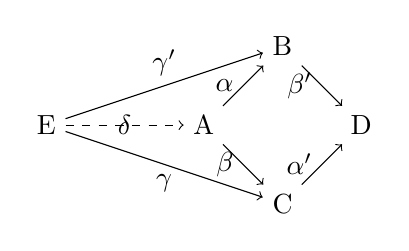
\begin{tikzpicture}
                        \node (i) at (0,0) {A};
                        \node (r) at (1,1) {B};
                        \node (c) at (1,-1) {C};
                        \node (h) at (2,0) {D}; 
                        % \node () at (1,-1) {\( \Delta \)};
                        \draw[->]  (i) -- (r) node [midway,left] {$\alpha$};
                        \draw[->] (c) -- (h) node [midway,left] {$\alpha'$};
                        \draw[->] (r) -- (h) node[midway, left] {$\beta'$};
                        \draw[->] (i) -- (c) node[midway, left] {$\beta$};
                        \node (d') at (-2,0) {E};
                        \draw[<-] (c) -- (d') node [midway,below]{$\gamma$};
                        \draw[<-] (r) -- (d') node [midway,above]{$\gamma'$};
                        \draw[->, dashed] (d') -- (i) node [midway]{$\delta$};
                    \end{tikzpicture}
        }
    %     \caption{}
    %     \label{fig:preliminaries:pullback_ssdsfd}
    % \end{figure}
                \end{center}
The diagram involving \( (\alpha, \beta, \alpha', \beta') \) is called a \textbf{pullback square}, or simply a \textbf{pullback}\index{Pullback!square}, with \(A\) as the \textbf{pullback object}\index{Pullback!object}. The existence of a unique morphism is known as the \textbf{universal mapping property of the pullback}\index{Pullback!universal mapping property}.
\end{definition} 

\begin{example} 
    \label{ex:cat:pbfsdljkgjasssss}
    In the category \textbf{Set},
    the pullback 
    of a cospan \(B \overset{\beta'}{\rightarrow} D \overset{\alpha'}{\leftarrow} C \) is the span \( B \overset{\alpha}{\leftarrow} A \overset{\beta}{\rightarrow} C \) where
    the pullback object is the set $A \mathop{=} \set{(b,c)\in B \mathop{\times} C \mathop{\mid} \beta (c) \mathop{=} \alpha (b)}$; $\alpha$ and $\beta$ are defined as the corresponding projections, e.g., $\alpha((b, c)) \mathop{=} b$ and $\beta((b, c)) \mathop{=} c$.
    Consider the following diagram in the category \textbf{Set}, where 
    sets are drawn as boxes,
    circles represent elements of sets, and numbers inside circles indicate how the functions map those elements.
    \begin{center}
      \resizebox{0.7\textwidth}{!}{
      \begin{tikzpicture}
          \graphbox{\( A\)}{40mm}{-3mm}{34mm}{12mm}{2mm}{2mm}{
              \coordinate (o) at (0mm,-8mm); 
              \node[draw,circle] (l1) at ($(o)+(-10mm,0mm)$) {1};
              \node[draw,circle] (l2) at ($(l1)+(2,0)$) {2};
          }  
          \graphbox{\( B \)}{80mm}{-3mm}{45mm}{12mm}{2mm}{2mm}{
              \coordinate (o) at (-5mm,-8mm); 
              \node[draw,circle] (l1) at ($(o)+(-10mm,0mm)$) {1};
              \node[draw,circle] (l2) at ($(l1)+(3,0)$) {2};
              \node[draw,circle] (l3) at ($(l1)+(1,0)$) {4};
            %   \node[draw,circle] (l4) at ($(l1)+(2,0)$) {5};
            %   \draw[ ] (l1) -- (l3) node[midway,above] {$a$};
            %   \draw[ ] (l3) -- (l4) node[midway,above] {$b$};
            %   \draw[ ] (l4) -- (l2) node[midway,above] {$a$};
          }     
          \graphbox{\( C  \)}{40mm}{-22mm}{34mm}{22mm}{2mm}{-3mm}{
              \coordinate (o) at (0mm,-3mm); 
              \node[draw,circle] (l1) at ($(o)+(-10mm,0mm)$) {1};
              \node[draw,circle] (l2) at ($(l1)+(2,0)$) {2};
            %   \node[draw,circle] (l4) at ($(l2)+(0,-1)$) {6};
              \node[ draw,circle] (l6) at ($(l1)+(0,-1)$) {3};
            %   \draw[ ] (l1) -- (l6) node[midway,left] {$a$};
            %   \draw[ ] (l2) -- (l4) node[midway,right] {$a$};
          }    
          \graphbox{\( D \)}{80mm}{-22mm}{45mm}{22mm}{2mm}{-3mm}{
              \coordinate (o) at (-5mm,-3mm); 
              \node[draw,circle] (l1) at ($(o)+(-10mm,0mm)$) {1};
              \node[draw,circle] (l2) at ($(l1)+(3,0)$) {2};
              \node[draw,circle] (l3) at ($(l1)+(1,0)$) {4};
            %   \node[draw,circle] (l4) at ($(l1)+(2,0)$) {5};
            %   \node[ draw,circle] (l5) at ($(l2)+(0,-1)$) {6};
              \node[ draw,circle] (l6) at ($(l1)+(0,-1)$) {3};
            %   \draw[ ] (l1) -- (l6) node[midway,left] {$a$};
            %   \draw[] (l1) -- (l3) node[midway,above] {$a$};
            %   \draw[] (l3) -- (l4) node[midway,above] {$b$};
            %   \draw[ ] (l4) -- (l2) node[midway,above] {$a$};
            %   \draw[ ] (l2) -- (l5) node[midway,right] {$a$};
          }    
          \node () at (77mm,-8mm) {\( \overset{\alpha}{\rightarrow} \)};
          \node () at (58mm,-18mm) {\( \beta\downarrow \)};
          \node () at (102mm,-18mm) {\( \beta'\downarrow \)};
          \node () at (77mm,-33mm) {\( \overset{\alpha'}{\rightarrow} \)};
      \end{tikzpicture}
      }
    \end{center} 
    The span \( B \overset{\alpha}{\leftarrow} A \overset{\beta}{\rightarrow} C \)
    % shown in Figure~\ref{fig:preliminaries:a_rewriting_step_dfjalsdkdfsdfjflg} 
    is the pullback of the cospan \(B \overset{\beta'}{\rightarrow} D \overset{\alpha'}{\leftarrow} C \).
    Indeed, the pullback object can be taken as the set $A' \mathop{=} \set{(1_B,1_C),(2_B,2_C)} \mathop{\subseteq} B \mathop{\times} C$, and the morphisms $\alpha'' \mathop{\colon} A'  \mathop{\to} B$ and $\beta'' \mathop{\colon} A'  \mathop{\to} C$ are defined as the corresponding projections, e.g., $\alpha''((x,y)) \mathop{=} x$ and $\beta''((x,y)) \mathop{=} y$. Note that $A$ is isomorphic to $A'$, which is expected because the pullback of a cospan is unique up to isomorphism.
\end{example}
In the category \textbf{Graph} pullbacks always exist and are computed pointwise: take the pullback in \textbf{Set} of the node sets and of the edge sets, and equip the resulting graph with source, target and labeling maps induced componentwise; the projection graph homomorphisms are the corresponding componentwise projections and they satisfy the universal property.
\begin{example}
    \label{ex:cat:pbfsdljkgjasssss2222ssss}
    Consider the diagram in the category \textbf{Graph}, shown below. The numbers inside nodes and the subgraphs in different colors illustrate how the morphisms map nodes and edges. 
    The span $L \overset{\alpha}{\leftarrow} K \overset{\beta}{\rightarrow} C$ is a pullback of the cospan $L \overset{\beta'}{\rightarrow} G \overset{\alpha'}{\leftarrow} C$.
    % \begin{figure}[H]
    %     \centering
    \begin{center}
        \resizebox{0.8\textwidth}{!}{
        \begin{tikzpicture} 
            \graphbox{\( L \)}{40mm}{20mm}{34mm}{20mm}{2mm}{2mm}{
                \coordinate (o) at (0mm,-10mm); 
                \node[draw,circle] (l1) at ($(o)+(-10mm,0mm)$) {1};
                \node[draw,circle] (l2) at ($(l1)+(2,0)$) {2};
                \draw[->,red] (l2) edge[out=-135,in=-45]node[midway,below] {$a$} (l1) ;
                \node[draw,circle,red] (l3) at ($(l1)+(1,0)$) {3};
                \draw[->,red] (l1) -- (l3) node[midway,above] {$a$};
                \draw[->,red] (l3) -- (l2) node[midway,above] {$a$};
            } 
    
            \graphbox{\( K \)}{0mm}{0mm}{34mm}{12mm}{2mm}{2mm}{
                \coordinate (o) at (0mm,-8mm); 
                \node[draw,circle] (l1) at ($(o)+(-10mm,0mm)$) {1};
                \node[draw,circle] (l2) at ($(l1)+(2,0)$) {2};
            }  
            \graphbox{\(G  \)}{90mm}{10mm}{34mm}{40mm}{2mm}{-3mm}{
                \coordinate (o) at (0mm,-20mm); 
                 \node[draw,circle] (l1) at ($(o)+(0,0)$) {1\ 2};
                % \node[draw,circle] (l1) at ($(o)+(-10mm,0mm)$) {1};
                % \node[draw,circle] (l2) at ($(l1)+(2,0)$) {2};
                \draw[->,red] (l1) edge[loop below] node[midway, below] {$a$} (l1) ;
                \node[draw,circle,red] (l3) at ($(l1)+(0,1.4)$) {3};
                \node[draw,circle,blue] (l4) at ($(l1)+(1,-1)$) {6};
                \draw[->,red] (l1) edge[bend left] node[midway,left] {$a$} (l3);
                \draw[->,red] (l3) edge[bend left] node[midway,right] {$a$} (l1);
                \draw[->,blue] (l1) edge  node[midway,right] {$a$} (l4);
                \node[draw,circle,blue] (l6) at ($(l1)+(-1,-1)$) {7};
                \draw[<-,blue] (l1) edge node[midway,left] {$a$} (l6) ;
                % \draw[->,blue] (l1) edge[out=-135,in=-45]node[midway,below] {$a$} (l1) ;
            }   
     
            \graphbox{\( C \)}{40mm}{-12mm}{34mm}{24mm}{2mm}{-3mm}{
                \coordinate (o) at (0mm,-5mm); 
                \node[draw,circle] (l1) at ($(o)+(0,0)$) {1\ 2};
                % \node[draw,circle] (l2) at ($(l1)+(2,0)$) {2};
                \node[draw,circle,blue] (l4) at ($(l1)+(1,-1)$) {6};
                \draw[->,blue] (l1) -- (l4) node[midway,right] {$a$};
                % \draw[->,blue] (l1) edge[loop above] node[midway, above] {$a$} (l1) ;
                \node[ draw,circle,blue] (l6) at ($(l1)+(-1,-1)$) {7};
                \draw[<-,blue] (l1) -- (l6) node[midway,left] {$a$};
            }
            % K to L  
            \draw[>->] (17mm,5mm) -- node[above] {$\alpha$} (37mm,15mm);
            % C to G
            \draw[>->] (76mm,-28mm)-- node[below] {$\alpha'$} (88mm,-26mm) ;
            % K to C
            \draw[->] (17mm,-17mm) -- node[below] {$\beta$} (37mm,-28mm);
            % L to G 
            \draw[->] (76mm,16mm) -- node[above] {$\beta'$} (88mm,10mm);
            \node () at (57mm,-6mm) {$PB$};
        \end{tikzpicture}
        }
    \end{center}
\end{example} 
Consider the following diagram in the category \textbf{Graph}:\begin{center}
        \resizebox{0.8\textwidth}{!}{
        \begin{tikzpicture} 
            \graphbox{\( L \)}{40mm}{15mm}{34mm}{12mm}{2mm}{2mm}{
                \coordinate (o) at (0mm,-8mm); 
                \node[draw,circle] (l1) at ($(o)+(-10mm,0mm)$) {1};
                \node[draw,circle] (l2) at ($(l1)+(2,0)$) {2};
                \node[draw,circle,red] (l3) at ($(l1)+(1,0)$) {3};
                \draw[->,red] (l1) -- (l3) node[midway,above] {$a$};
                \draw[->,red] (l3) -- (l2) node[midway,above] {$a$};
            } 
    
            \graphbox{\( K \)}{0mm}{0mm}{34mm}{12mm}{2mm}{2mm}{
                \coordinate (o) at (0mm,-8mm); 
                \node[draw,circle] (l1) at ($(o)+(-10mm,0mm)$) {1};
                \node[draw,circle] (l2) at ($(l1)+(2,0)$) {2};
            }  
            \graphbox{\(G  \)}{90mm}{5mm}{34mm}{24mm}{2mm}{-3mm}{
                \coordinate (o) at (0mm,-5mm); 
                \node[draw,circle] (l1) at ($(o)+(-10mm,0mm)$) {1};
                \node[draw,circle] (l2) at ($(l1)+(2,0)$) {2};
                \node[draw,circle,red] (l3) at ($(l1)+(1,0)$) {3};
                \node[draw,circle,blue] (l4) at ($(l2)+(0,-1)$) {6};
                \draw[->,red] (l1) -- (l3) node[midway,above] {$a$};
                \draw[->,red] (l3) -- (l2) node[midway,above] {$a$};
                \draw[->,blue] (l2) -- (l4) node[midway,right] {$a$};
                \node[draw,circle,blue] (l6) at ($(l1)+(0,-1)$) {7};
                \draw[<-,blue] (l1) -- (l6) node[midway,left] {$a$};
                \draw[->,blue] (l2) edge[out=-135,in=-45]node[midway,below] {$a$} (l1) ;
            }   
     
            \graphbox{\( C \)}{40mm}{-15mm}{34mm}{24mm}{2mm}{-3mm}{
                \coordinate (o) at (0mm,-5mm); 
                \node[draw,circle] (l1) at ($(o)+(-10mm,0mm)$) {1};
                \node[draw,circle] (l2) at ($(l1)+(2,0)$) {2};
                \node[draw,circle,blue] (l4) at ($(l2)+(0,-1)$) {6};
                \draw[->,blue] (l2) -- (l4) node[midway,right] {$a$};
                \draw[->,blue] (l2) edge[out=-135,in=-45]node[midway,below] {$a$} (l1) ;
                \node[ draw,circle,blue] (l6) at ($(l1)+(0,-1)$) {7};
                \draw[<-,blue] (l1) -- (l6) node[midway,left] {$a$};
            }      
            % K to L
            \draw[>->] (17mm,5mm) -- node[above] {$\alpha$} (37mm,10mm);
            % C to G
            \draw[>->] (76mm,-28mm)-- node[below] {$\alpha'$} (104mm,-21mm) ;
            % K to C
            \draw[>->] (17mm,-17mm) -- node[below] {$\beta$} (37mm,-28mm);
            % L to G
            \draw[>->] (76mm,10mm) -- node[above] {$\beta'$} (104mm,7mm);
            \node () at (57mm,-6mm) {$PO$};
        \end{tikzpicture}
        }
    \end{center}
We observe that it is a pushout square as well as a pullback square. This is not a coincidence, as stated in the following proposition.
\begin{proposition}[\text{\cite[Lemma 13]{lack2004adhesive}}]
    \label{prop:pb_eq_po}
    In the category \textbf{Graph}, pushouts along monomorphisms are also pullbacks. 
\end{proposition}
This proposition is illustrated in Example~\ref{ex:cat:pushout_non_injective_ssss} and Example~\ref{ex:cat:pbfsdljkgjasssss2222ssss}.

\begin{definition}[Pullback \cite{pierce1991basic}]
    \label{def:cat:pb}
    \ \newline
\noindent
\begin{minipage}{0.7\textwidth}  
   A \textbf{pullback} of a cospan \(B \overset{\beta'}{\rightarrow} D \overset{\alpha'}{\leftarrow} C \), as shown on the right, is defined as a span \( B \overset{\alpha}{\leftarrow} A \overset{\beta}{\rightarrow} C \) such that \( \alpha \star \beta' = \beta \star \alpha' \), and for every span \( B \overset{\gamma'}{\leftarrow} E \overset{\gamma}{\rightarrow} C \) if \(\gamma' \star \beta' = \gamma \star \alpha'\) holds, then there exists a unique morphism \(\delta: E \to A\) such that $\gamma' = \delta \star \alpha$ and $\gamma = \delta \star \beta$. 
\end{minipage}
\hfill
\begin{minipage}{0.299\textwidth}
    \hfill
\resizebox{0.9\textwidth}{!}{
            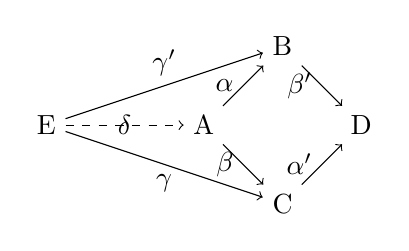
\begin{tikzpicture}
                \node (i) at (0,0) {A};
                \node (r) at (1,1) {B};
                \node (c) at (1,-1) {C};
                \node (h) at (2,0) {D};
                % \node () at (1,-1) {\( \Delta \)};
                \draw[->]  (i) -- (r) node [midway,left] {$\alpha$};
                \draw[->] (c) -- (h) node [midway,left] {$\alpha'$};
                \draw[->] (r) -- (h) node[midway, left] {$\beta'$};
                \draw[->] (i) -- (c) node[midway, left] {$\beta$};
                \node (d') at (-2,0) {E};
                \draw[<-] (c) -- (d') node [midway,below]{$\gamma$};
                \draw[<-] (r) -- (d') node [midway,above]{$\gamma'$};
                \draw[->, dashed] (d') -- (i) node [midway]{$\delta$};
            \end{tikzpicture}
}
\end{minipage}
The diagram involving \(\alpha\), \(\beta\), \(\alpha'\), and \(\beta'\) is referred to as the \textbf{pullback square}, \(A\) as the \textbf{pullback object}, and the existence of the unique morphism is known as the \textbf{universal mapping property of the pullback}.
\end{definition} 
% In the category \(\mathbf{Graph}\) pushouts always exist, and their construction is straightforward when dealing with monomorphisms (injective graph homomorphisms). 
% Let $\uplus$ denote the disjoint union operation. For two sets \(A\) and \(B\), their disjoint union \(A \uplus B\) is defined as the set of ordered pairs \( (x, i) \) where \( x \mathop{\in} A \) if \( i \mathop{=} 1 \) and \( x \mathop{\in} B \) if \( i \mathop{=} 2 \). Formally, we have:
% $
% A \uplus B \mathop{=} \{ (x, 1) : x \mathop{\in} A \} \mathop{\cup} \{ (x, 2) : x \mathop{\in} B \}.
% $ 
We denote $X\uplus Y$ the union of two disjoint sets. By possibly renaming nodes, a span of injective graph homomorphisms can be represented as
$
A \uplus B' \overset{\alpha}{\leftarrowtail} A \overset{\beta}{\rightarrowtail} A \uplus C'
$
where $A,B',C'$ are disjoint sets and $\alpha$ and $\beta$ are inclusion function. A pushout of this span is then given by
$
A \uplus B'  \overset{\beta'}{\rightarrowtail} A \uplus B' \uplus C'   \overset{\alpha'}{\leftarrowtail} A \uplus C'
$ where $\alpha'$ and $\beta'$ are inclusion function. This situation can be depicted by the diagram in Figure~\ref{fig:po_decomp}
\begin{figure}[htbp] 
    \begin{center}
    \resizebox{0.45\textwidth}{!}{
        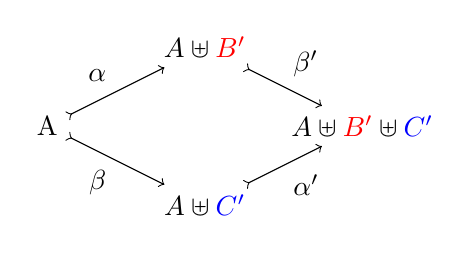
\begin{tikzpicture}
                    \node (i) at (0,0) {A};
                    \node (r) at (2,1) {$A \uplus \textcolor{red}{B'}$};
                    \node (c) at (2,-1) {$A \uplus \textcolor{blue}{C'}$};
                    \node (h) at (4,0) {$A \uplus \textcolor{red}{B'} \uplus \textcolor{blue}{C'}$};
                    \draw[>->]  (i) -- (r) node [midway, above left] {$\alpha$};
                    \draw[>->] (c) -- (h) node [midway, below right] {$\alpha'$};
                    \draw[>->] (r) -- (h) node[midway, above right] {$\beta'$};
                    \draw[>->] (i) -- (c) node[midway, below left] {$\beta$};
        \end{tikzpicture}
    }
    \end{center}
    
    \caption{Construction of the pushout of a span of monomorphisms in \(\mathbf{Graph}\)}
    \label{fig:po_decomp}
\end{figure}
where \(B'\) and \(C'\) are colored to make evident this decomposition in a concrete example within \textbf{Graph} in Example~\ref{ex:po_in_graph}, where nodes and arrows are colored accordingly.

% %po example in Graph
% \begin{example}
    \label{ex:po_in_graph}
    The following diagram
    %  in Figure~\ref{fig:ex:po_in_graph} 

% \begin{figure}[H] 
\begin{center}
    \resizebox{0.5\textwidth}{!}{
        \begin{tikzpicture}
               
                \graphbox{ }{40mm}{5mm}{34mm}{15mm}{2mm}{0mm}{
                    \coordinate (o) at (0mm,-8mm); 
                    \node[draw,circle] (l1) at ($(o)+(-10mm,0mm)$) {1};
                    \node[draw,circle] (l2) at ($(l1)+(2,0)$) {2};
                }  
  
                \graphbox{ }{80mm}{5mm}{45mm}{15mm}{2mm}{-0mm}{
                    \coordinate (o) at (-5mm,-8mm); 
                    \node[draw,circle] (l1) at ($(o)+(-10mm,0mm)$) {1};
                    \node[draw,circle] (l2) at ($(l1)+(3,0)$) {2};
                    \node[red,draw,circle] (l3) at ($(l1)+(1,0)$) {4};
                    \node[red,draw,circle] (l4) at ($(l1)+(2,0)$) {5};
                    \draw[red] (l1) -- (l3) node[midway,above] {$a$};
                    \draw[red] (l3) -- (l4) node[midway,above] {$b$};
                    \draw[red] (l4) -- (l2) node[midway,above] {$a$};
                }    
                \graphbox{ }{40mm}{-17mm}{34mm}{25mm}{2mm}{-5mm}{
                    \coordinate (o) at (0mm,-3mm); 
                    \node[draw,circle] (l1) at ($(o)+(-10mm,0mm)$) {1};
                    \node[draw,circle] (l2) at ($(l1)+(2,0)$) {2};
                    \node[blue,draw,circle] (l4) at ($(l2)+(0,-1)$) {6};
                    \draw[blue] (l2) -- (l4) node[midway,right] {$a$};
                    \node[blue,draw,circle] (l6) at ($(l1)+(0,-1)$) {7};
                    \draw[blue] (l1) -- (l6) node[midway,left] {$a$};
                }    
  
                \graphbox{ }{80mm}{-17mm}{45mm}{25mm}{2mm}{-5mm}{
                    \coordinate (o) at (-5mm,-3mm); 
                    \node[draw,circle] (l1) at ($(o)+(-10mm,0mm)$) {1};
                    \node[draw,circle] (l2) at ($(l1)+(3,0)$) {2};
                    \node[draw,circle,red] (l3) at ($(l1)+(1,0)$) {4};
                    \node[draw,circle,red] (l4) at ($(l1)+(2,0)$) {5};
                    \node[blue,draw,circle] (l5) at ($(l2)+(0,-1)$) {6};
                    \node[blue,draw,circle] (l6) at ($(l1)+(0,-1)$) {7};
                    \draw[blue] (l1) -- (l6) node[midway,left] {$a$};
                    \draw[red] (l1) -- (l3) node[midway,above] {$a$};
                    \draw[red] (l3) -- (l4) node[midway,above] {$b$};
                    \draw[red] (l4) -- (l2) node[midway,above] {$a$};
                    \draw[blue] (l2) -- (l5) node[midway,right] {$a$};
                }    
  
                \node () at (77mm,-3mm) {\( \rightarrowtail \)}; % K -> R
                \node () at (52mm,-13mm) {\( \downarrowtail \)};
                \node () at (92mm,-13mm) {\( \downarrowtail \)};
                \node () at (77mm,-28mm) {\( \rightarrowtail \)}; % C -> H
        \end{tikzpicture}
    }
\end{center}
% \caption{Example of the pushout of span of monomorphism in \(\mathbf{Graph}\)}
% \label{fig:ex:po_in_graph}
% \end{figure}
     is a pushout square in the category \textbf{Graph} where nodes and arrows are colored to visualize the decomposition as in Figure~\ref{fig:po_decomp}.
\end{example}

To demonstrate that the diagram above is a pushout square, consider an object \( X \) and morphisms \( f: A \uplus B' \mathop{\to} X \) and \( g: A \uplus C' \mathop{\to} X \) such that \( \alpha \mathop{\star} f \mathop{=} \beta \mathop{\star} g \). Since \( \alpha \) and \( \beta \) are inclusion maps, it follows that \( f \) and \( g \) agree on \( A \). Therefore, the morphism \( h: A \uplus B' \uplus C' \mathop{\to} X \) defined by $h(x) \mathop{=} f(x)$ if $x\in A\uplus B'$ and $h(x) \mathop{=} g(x)$ otherwise is the unique morphism such that $\beta' \mathop{\star} h \mathop{=} f$ and $\alpha' \mathop{\star} h \mathop{=} g$. Thus, the object \( A \uplus B' \uplus C' \), together with the morphisms \( \beta' \) and \( \alpha' \), satisfies the universal property of the pushout. Furthermore, the compositions \( \alpha \mathop{\star} \beta'\) and \( \beta \mathop{\star} \alpha'\) both map elements from \( A \) to \( A \uplus B' \uplus C' \) via inclusion function.
Since all maps are inclusions and \( A \), \( B' \), and \( C' \) are disjoint, the square commutes $
     \alpha \mathop{\star} \beta' \mathop{=} \beta \mathop{\star} \alpha'
$. Therefore, the diagram is indeed a pushout square.
%pb po in Grap
\begin{notation}
    When the context makes it clear, a morphism \( h : A \to B \) will be denoted by \( h_{AB} \), and diagrams will be referred to by their nodes, as is standard in geometry. For example, the diagram involving the morphisms \( \alpha, \beta, \alpha', \beta' \) in~\autoref{def:cat:po} will be denoted by \( ACDB \) or \( ABDC \).
\end{notation}   
\begin{remark}
    We work within the category \textbf{Graph}. The terms homomorphism and morphism will be used interchangeably; the same applies to monic and injective, and to injective homomorphism and monomorphism.
\end{remark}